


\tikzset{every picture/.style={line width=0.75pt}} %set default line width to 0.75pt

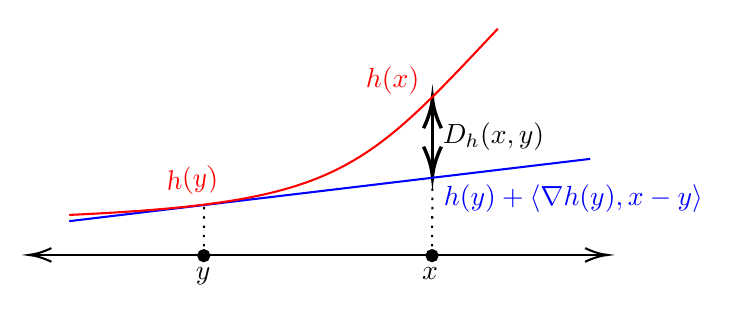
\begin{tikzpicture}[x=0.75pt,y=0.75pt,yscale=-1,xscale=1]
%uncomment if require: \path (0,308); %set diagram left start at 0, and has height of 308

%Straight Lines [id:da8132100594867722]
\draw    (73,200.33) -- (348,200.33) ;
\draw [shift={(350,200.33)}, rotate = 180] [color={rgb, 255:red, 0; green, 0; blue, 0 }  ][line width=0.75]    (10.93,-3.29) .. controls (6.95,-1.4) and (3.31,-0.3) .. (0,0) .. controls (3.31,0.3) and (6.95,1.4) .. (10.93,3.29)   ;
\draw [shift={(71,200.33)}, rotate = 0] [color={rgb, 255:red, 0; green, 0; blue, 0 }  ][line width=0.75]    (10.93,-3.29) .. controls (6.95,-1.4) and (3.31,-0.3) .. (0,0) .. controls (3.31,0.3) and (6.95,1.4) .. (10.93,3.29)   ;
%Shape: Circle [id:dp9237316574850754]
\draw  [fill={rgb, 255:red, 0; green, 0; blue, 0 }  ,fill opacity=1 ] (262.67,200.67) .. controls (262.67,199.19) and (263.86,198) .. (265.33,198) .. controls (266.81,198) and (268,199.19) .. (268,200.67) .. controls (268,202.14) and (266.81,203.33) .. (265.33,203.33) .. controls (263.86,203.33) and (262.67,202.14) .. (262.67,200.67) -- cycle ;
%Shape: Circle [id:dp045787056716331875]
\draw  [fill={rgb, 255:red, 0; green, 0; blue, 0 }  ,fill opacity=1 ] (152.67,200.67) .. controls (152.67,199.19) and (153.86,198) .. (155.33,198) .. controls (156.81,198) and (158,199.19) .. (158,200.67) .. controls (158,202.14) and (156.81,203.33) .. (155.33,203.33) .. controls (153.86,203.33) and (152.67,202.14) .. (152.67,200.67) -- cycle ;
%Straight Lines [id:da4276666085658716]
\draw  [dash pattern={on 0.84pt off 2.51pt}]  (155.33,200.67) -- (155.52,176.05) ;
%Straight Lines [id:da6234026284865279]
\draw  [dash pattern={on 0.84pt off 2.51pt}]  (265.33,200.67) -- (265.52,162.38) ;
%Straight Lines [id:da22897635371079694]
\draw [line width=1.25]    (265.52,159.38) -- (265.52,128.05) ;
\draw [shift={(265.52,125.05)}, rotate = 450] [color={rgb, 255:red, 0; green, 0; blue, 0 }  ][line width=1.25]    (14.21,-4.28) .. controls (9.04,-1.82) and (4.3,-0.39) .. (0,0) .. controls (4.3,0.39) and (9.04,1.82) .. (14.21,4.28)   ;
\draw [shift={(265.52,162.38)}, rotate = 270] [color={rgb, 255:red, 0; green, 0; blue, 0 }  ][line width=1.25]    (14.21,-4.28) .. controls (9.04,-1.82) and (4.3,-0.39) .. (0,0) .. controls (4.3,0.39) and (9.04,1.82) .. (14.21,4.28)   ;
%Straight Lines [id:da4257640445897286]
\draw [color=blue  ,draw opacity=1 ]   (90.52,184.05) -- (341.52,154.05) ;
%Curve Lines [id:da37061921880533877]
\draw [color=red  ,draw opacity=1 ][line width=0.75]    (90.52,181.05) .. controls (219.52,175.05) and (231.52,161.05) .. (297,91.33) ;

% Text Node
\draw (150,205) node [anchor=north west][inner sep=0.75pt]    {$y$};
% Text Node
\draw (259,205) node [anchor=north west][inner sep=0.75pt]    {$x$};
% Text Node
\draw (134.94,158) node [anchor=north west][inner sep=0.75pt]  [color=red  ,opacity=1 ,rotate=-353.99]  {$h( y)$};
% Text Node
\draw (232,108) node [anchor=north west][inner sep=0.75pt]  [color=red  ,opacity=1 ]  {$h( x)$};
% Text Node
\draw (269,135) node [anchor=north west][inner sep=0.75pt]    {$D_{h}( x,y)$};
% Text Node
\draw (269.52,165) node [anchor=north west][inner sep=0.75pt]  [color=blue  ,opacity=1 ]  {$h( y) +\langle \nabla h( y) ,x-y\rangle $};


\end{tikzpicture}
